\chapter{如何改善敏捷开发质量} % Introduction chapter suppressed from the table of contents


\framebox{%
\begin{minipage}[t]{0.97\columnwidth}\raggedright
按瀑布式阶段开发的困难:\\毕业后参加的开发项目,客户是电信行业,很规范,所以有一定的里程碑和阶段要求。有分析阶段、设计阶段、编码阶段,最后交付,里面当然包括一些测试。\\但往往因为客户的需求不断变化,每一两周都会有新的要求,因为电信业面对的市场变化也很大。导致本来我们预计六个月的项目,后面会有三到四周的测试和调试。也因为不断的有需求变化,不断在修改,几乎就没有时间做好测试,导致为了赶本来合同规定的交付时间,后期不准熬夜加班,更惨的是没来得及测试好,很多代码还是有不少缺陷。\\ 其中一个原因,如果可以把本来前面的设计画UML图的时间省略掉,应该可以腾出更好的时间来做后面的开发和测试。所以当张工开始接触敏捷开发,很相信这种快速交付迭代的方式可以对团队有帮助。\strut
\end{minipage}}

\hypertarget{ux67d0ux8f6fux4ef6ux5f00ux53d1ux516cux53f8ux654fux6377ux5f00ux53d1ux8fc7ux7a0bux6539ux8fdbux6848ux4f8b}{%
\subsection{某软件开发公司敏捷开发过程改进案例}\label{ux67d0ux8f6fux4ef6ux5f00ux53d1ux516cux53f8ux654fux6377ux5f00ux53d1ux8fc7ux7a0bux6539ux8fdbux6848ux4f8b}}

\hypertarget{ux6708}{%
\subsubsection{5月}\label{ux6708}}

张工是公司的中层管理,管理好几个开发团队,有五位项目经理向他汇报。\\
他听说老同学的团队都开始用敏捷开发,很感兴趣,并参加了一些敏捷的交流会,觉得可以解决很多传统瀑布性开发的不足,尤其是可以快速交付给客户。\\
他要求部门经理全面推动敏捷开发,对团队成员进行相关培训,例如,SCRUM Master 内部培训。\\
开始时,张工上级部门经理有些怀疑,问:“后面那些工程文档都不做,会不会影响质量和交付?客户都是专门做电信的,不缺钱,但是对质量要求很高。”\\
张工便解释说,“只要利用敏捷把过程变成迭代,快速交付,改善工程的问题不难,主要是人的问题。”\\
部门经理听到敏捷可以比以前更快速交付,之前客户经常因为延误而不满,他希望可以改变这现状,就答应了。 \\

\hypertarget{ux6708-1}{%
\subsubsection{8月}\label{ux6708-1}}

开发组长王工周五下班后与朋友喝酒,开开心心说: “太兴奋了。研发部门经理决定全面推动敏捷开发SCRUM;我们团队刚参加了两天培训,真正对应我们以前的传统瀑布式开发的种种问题,我们会2周一次迭代,快速反馈,我们会定期小步向客户发版,我们会与用户经常交流,获得他们的反馈。\\
现在团队合作不像以前只按工种工作,也会跟产品经理、业务方面更充分合作,给客户带来更高价值。\\
工作方式也改变了,以前要写需求、规格说明书,现在简单化成用户故事和产品需求卡片,以前我们要做过详细项目计划甘特图,现在用改成用燃烧图和白板。每天用便利贴去写要开发什么东西贴在白板上面,开始的时候,贴的越多感觉越敏捷,我们改成叫 SCRUM team,有一系列的海报围绕我们。我们也没项目经理了,自己管理自己。本来的部门经理现在变成产品负责人,敏捷开发方式让我们团队自己做决策,不仅仅是技术方面,项目相关的也由我们项目组一起讨论决定。\\
解除了以前‘瀑布式开发’的种种烦恼,这一切太完美了。“\\

\hypertarget{ux6708-2}{%
\subsubsection{9月}\label{ux6708-2}}

”你们团队学完敏捷SCRUM后,项目如何?”\\
王工充满自豪地说:\\
“我们培训后就SCRUM的方法,定每两周一个冲刺,每次冲刺前都会用故事点来估算每个功能多大,然后按本次冲刺的资源,估计可以完成多少功能?\\
然后用白板来监控模块完成的情况,哪些在开发中,哪些已经完成,团队和管理者都可以一目了然,不用像以前天天问我们了。我们每天早上也按照SCRUM的规定站立会议,每人说自己完成了哪些任务,今天做什么。\\
大家都很兴奋,确实跟以前瀑布的做法不同。”\\

\hypertarget{ux6708-3}{%
\subsubsection{10月}\label{ux6708-3}}

”你们项目如何?”\\
王工听完,想了一下,然后说:\\
“我们本应上周要完成一次冲刺后的割接上线,但被推到下次了。“\\
”为什么?”\\
王工说: ”我们按培训学到的做冲刺计划会,按照产品的待办事项列表,团队利用扑克牌一起估算每一事项所需要的时间。我们总共八位开发人员,其中有一半是刚毕业不久,但大家刚上完培训,很有信心,虽然技术主管张工对我们出来的估算有些顾虑,觉得我们太理想,但大家刚培训完敏捷,张工也希望让部门经理尽快看到敏捷开发可以加快速度,我们就按这‘进取式’估算开展2周冲刺。\\
但因新人多,编码水平有限,虽然大家已经尽快把开发出来的代码交给系统测试人员手工测试,依据测试发现的缺陷修正再测试,但越来越接近答应客户的2周割接上线时间,但是还是很多BUG没改好,最后几天,基本就天天加班,最终到验收时,仍然有不少问题,最终割接前测试,还是不能达到客户要求的水平,没办法,未能上线。\\
大家确实都尽力冲刺了,但未能达到我们本来希望的结果。“ \\

\hypertarget{ux6708-4}{%
\subsubsection{11月}\label{ux6708-4}}

部门经理之前收到客户总监电话,投诉一些技术缺陷,导致好几次不能按计划上线,问为什么正在交付的软件质量变差了?\\

张工被问到是什么原因时无法回答,只能说立马回去探索原因,尽快汇报,但心里想: “开始敏捷后,因为快速迭代,以前要做概要设计、详细设计的过程反而被忽略了,导致有些写出来的代码,后面就很很难适应快速的变化修改,导致要不然就功能做不出来。 因要赶时间,可以按客户的要求时间交付的话,由于本身代码不好,只可以临时凑凑,不长久。”\\
张工从部门经理办公室出来后,找其中一位项目经理李工喝茶,回顾一下发现项目团队对这次敏捷SCRUM的改革有意见。例如上层为了更快速交付,实现敏捷可以快速交付承诺,把一些本来不太可能的进度时间压到团队去,完全不是本来的那种自主团队管理的概念。出现问题多了,就请了敏捷教练过来辅导,但SCRUM的教练也缺乏软件工程的基础,只懂项目管理过程。所以他们也解决不了软件相关的问题。只是把精益管理怎么做迭代,怎么做回顾这些基本过程再解读一下,解决不了实际问题。\\

李工:
”因为我们做这块业务已经很多年了,本来业务的变化不多,只是一些小的功能改动,所以开发人员尽量不去动核心的代码,怕改动了反而会影响投产,切割不了。但有时为了满足一些新功能,继续在老代码的基础上去写,这种做法效率很低,也不长久,估计一两年后会难以运行了,我们会被迫重写整个产品,而老代码开发人员大部分都离开了,后面的代码维护变得非常困难,即使用敏捷也解决不了这个问题。”\\

无论张工或李工也没有能去总结出什么好的解决方案。现在推行敏捷才刚刚三个月,绝不能打退堂鼓,回到本来的状态。但应怎么解决敏捷带来的问题?挽回部门经理与客户的信心呢?\\
\hypertarget{ux5982ux4f55ux6539ux5584}{%
\subsection{如何改善}\label{ux5982ux4f55ux6539ux5584}}

从以上案例看到,本来管理层希望利用敏捷开发,加快软件开发的交付,减少延误,令客户更满意。但因为只注重项目管理,但没注意和改善软件开发本身的质量,人员能力等因素,开发出来的软件缺陷比以往多,导致后面大量返工,恶性循环,后面更导致延误,最终客户投诉。\\
因为软件本身设计有问题,导致软件难以修改,开发人员都不敢改动任何代码,怕可能会引起系统崩溃。\\

怎样可以确保开发出来软件的质量?\\

敏捷开发有很多种方法(SCRUM 只是其一),因为目的不仅仅是管好项目进度,也要确保软件产品的质量。所以SCRUM 只包括项目管理部分,不全面,反过来,例如极限编程(XP eXtreme Programming),因它的发明者Kent BECK 本身是一位精通面向对象的编程员,所以XP不仅仅关注项目管理,也包含编程的最佳实践。下图是 Ron Jeffery 把XP的重点画成从外到内3层: \\

%\href{文件:cleanagile_f1.8.jpg}{500px}。


\includegraphics[width=10cm]{cleanagile_f18.jpg}

SCRUM 只包含了外层的部分,缺乏中间和内层元素。
按XP的12实践(详见附件)都做到了便可以解决张工的问题吗?\\
不一定。

\framebox{%
\begin{minipage}[t]{0.97\columnwidth}\raggedright Dr
Juran,德鲁克(Drucker)和戴明(Deming)博士是同代人,出生日期相差不超过十年,他们3位都在战后去过日本,帮助日本企业家改善他们的质量。\\在50年代,当德鲁克被ASQ记者问为什么他声称Dr
Juran是现代生产管理之父?\\ 德鲁克解释说:\\现在我们常用的精益(Lean)生产和JIT,其实都是源自Joe
(Joseph Juran)
的过程管理思路,他一直主张要从工作过程入手,从产出反过来决定过程应该如何配合。虽然他没有用"精益"这个词,但他很明白要管理好生产,必须以如何使工人能最好发挥为本,但他这思路被美国很多学术界人士和工业工程师反对:``为什么不是应该由管理者做主,生产者反而成为主角?''\\ 其实戴明、Joe和我都很理解从上而下那一套管理方式是行不通的。日本战后急于回复经济,很接受我们的管理思路,并立马执行,例如丰田40年代未开始推JIT,赶上并超越美国的工业生产。比如我一直和通用汽车(GM)有交流,发现他们就不懂必须先梳理好过程这个概念,从产出反推生产过程应如何配合。尽管GM投入数以亿计的资金自动化信息化,希望改善机器及物流管理,但却不知道本应从过程入手,导致生产到今天也无法追上日本(那套JIT的汽车生产模式)。虽然Joe的思路很清晰,也知道怎么改进企业的质量,可惜一直默默耕耘,没有受到该有的重视。\\ 注:ASQ=American
Society of Quality; JIT=Just-In-Time\strut
\end{minipage}}


下面我们回顾质量大师Dr JURAN 的质量策划方式,如何提升产品质量。\\
客户问:你说Juran先生?\\
我:是的。\\
客户:会不会他的那套质量改进方法太老了,不适用于我们现代。而且他主要关注制作业,不太熟悉我们IT业。\\
我:你听过乔布斯吗?\\
客户:当然听过了,他是苹果创始人。\\
我:乔布斯被苹果赶出来后,自己开创NEXT公司,希望创作未来新一代的电脑产品。他很希望产品在质量方面比较出众。当时,他觉得美国很多企业家都忽略了质量,感觉到被日本的竞争对手赶上。乔布斯便邀请了Dr
Juran从美国东岸飞到西岸,帮他的NEXT公司做辅导,改进过程。(关于他对Dr
Juran的评价,详见附件)

%\href{文件:jobs1Screenshot_2022-06-12_082703.jpg}{100px\textbar{}缩略图}

\includegraphics[width=10cm]{jobs1Screenshot_2022-06-12_082703.jpg}

后面乔布斯回到苹果,大部分NEXT工程师也跟着他一起进入苹果。所以我们现在用一些苹果产品,多多少少都会受当时NEXT质量改进的影响。

我:首先要定义质量是什么?\\

\framebox{%
\begin{minipage}[t]{0.97\columnwidth}\raggedright
质量包括两部分:

\begin{description}
\tightlist
\item[]
满足客户需要 (客户包括外部客户和内部客户)

没有缺陷\\
\end{description}

这定义不仅仅适合于制作业、也适用于服务业,IT业。\\
\strut
\end{minipage}}



我:记得您比较懂财务,对吗?\\
客户:是的,其实我对软件开发还是外行,但较了解财务。\\
我:财务管理是不是包括财务策划、财务监控,财务改进?\\
客户:是的\\
我:Dr
Juran就用财务管理比喻质量管理,同样也有质量策划、质量控制和质量改进。你觉得这个大框架再细分要如何制定质量目标,如何来制定度量等。

%\href{文件:finAnalogyScreenshot_2022-10-07_212149.jpg}{文件:finAnalogyScreenshot
%2022-10-07 212149.jpg}

\includegraphics[width=10cm]{finAnalogyScreenshot_2022-10-07_212149.jpg}

从下表可以看得出来。所以如果我们希望利用敏捷开发,不仅仅是走迭代,确保进度没偏差,还要确保软件产品的质量,也应该用Dr
Juran的质量管理框架去看整个敏捷过程,才能更全面了解如何才可以确保软件开发的质量,也控制好交付工期,不延误,让客户满意。\\
质量策划还包括:

\begin{enumerate}
\tightlist
\item
  设定目标,包括外部和内部目标
\item
  识别内部需求
\item
  依据客户需求制定产品的功能特征
\item
  制定产品和过程的目标
\item
  设计过程来达到这些目标,最后验证过程能力\\
\end{enumerate}

可以用下图了解质量控制和质量改进,比如图的左面就是在过程之前的策划部分。如我们发现缺陷比率为20\%,这就是过程的能力,这个能力是策划的时候已经定好的,过程控制没有什么可以做,只是当缺陷有变化,比如特别高的时候,需要做一些措施返回本来的水平。要改进必须用质量改进,比如希望把缺陷百分比从20\%降到3\%,这就必须驱动一系列的改进计划。改进计划必须要按项目推行执行,没有其它办法。\\
%\href{文件:JuranImprovementScreenshot_2022-10-23_211444.jpg}{500px}

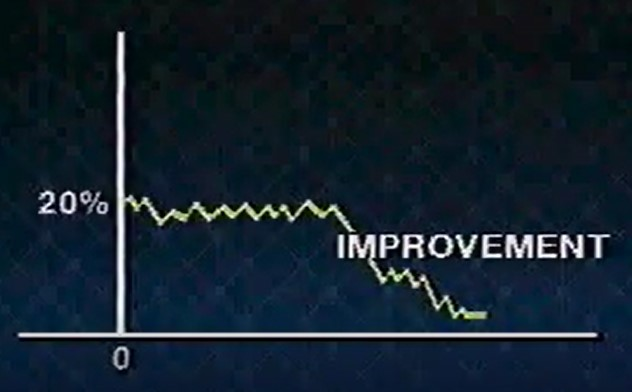
\includegraphics[width=10cm]{JuranImprovementScreenshot_2022-10-23_211444.jpg}

过程改进的计划一般包括:

\begin{enumerate}
\tightlist
\item
  如何识别选择项目。
\item
  组织改进项目的项目团队
\item
  找出缺陷根因
\item
  制定改进措施
\item
  验证是否在真正操作环境里面有效
\item
  处理团队文化上面的抗击阻力
\item
  控制保持本来的水平\\
\end{enumerate}

%\href{文件:IntroXPnJuranStepsScreenshot_2022-10-27_194505.jpg}{550px}

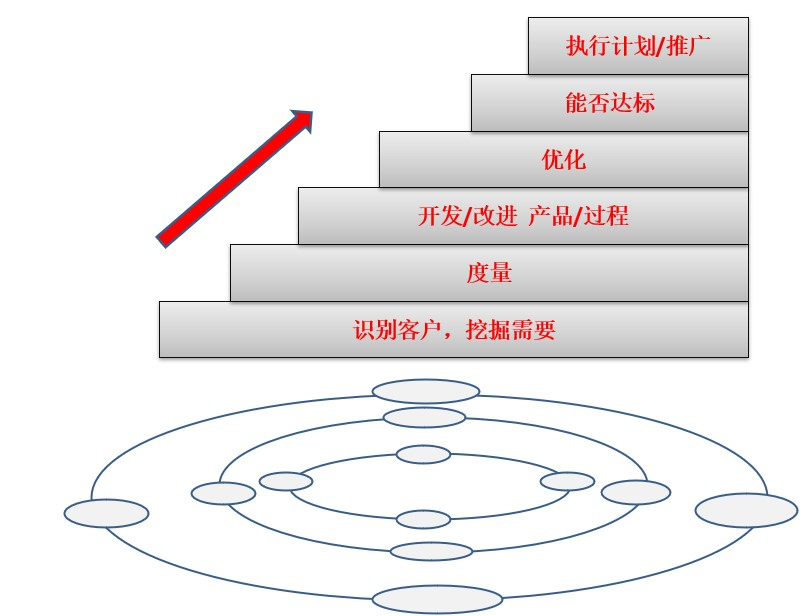
\includegraphics[width=10cm]{IntroXPnJuranStepsScreenshot_2022-10-27_194505.jpg}

客户:你说的策划、控制、改进都挺有道理,但如何跟敏捷,尤其是你说极限编程的实践关联呢?\\
我:任何最佳实践,如果没有定质量目标,配上度量衡量和策划,都只是空想,对长远提升公司文化、团队成员的习惯没有任何帮助。举例:参照上图,例如我们想改善团队的策划和估算。首先要识别客户,哪些是主要干系人
-
甲方有什么要求;内部部门经理,有什么要求。然后从他们的诉求变成过程的功能和特征,但如果特征只是描述,没有数字也没有意义,所以要配合可衡量的度量单位,和用什么方式去收集那些数字,然后依据目标定过程要怎么去做,怎样改。例如

\begin{itemize}
\tightlist
\item
  是否应该从本来的瀑布策划方式制定大的总计划,改用精益的思路,分成迭代,
\item
  每次估算应该怎么做、如何监控等
\item
  然后改进的过程要不断从实验中优化
\item
  最后还要用数字证明这改善比本来好,然后在其他团队全面推广\\
\end{itemize}

而不是单纯`空降'某敏捷流程(例如 SCRUM),便能加快团队的发布速度。
所以虽然极限编程里每一条实践都是最佳实践,也必须配合质量策划,和监控改进才会有效果。

\framebox{%
\begin{minipage}[t]{0.97\columnwidth}\raggedright
很多人都知道戴明环代表PDCA(Plan-Do-Check-Act),其实持续改进的道理也不是戴明博士发明,Juran
对它的了解与应用不会比戴明差。\strut
\end{minipage}}

要注意在整个过程里,高层起非常关键的作用:\\
所以Dr
Juran强调高层不能把公司的质量工作下放(例如,由某助手负责)。我们的经验就是这种做法往往导致最后质量不会有任何改进。原因很简单,每位中层管理者都有一定的KPI标准,资源也是固定的。如果这些没有根本的改变,质量是不会提升,因为整个管理环境没有变化,项目经理、部门经理还是会按以前的做法继续操作,不会听高层的口号或宣传,很快整个质量改进将会失败而终,所有的活动尤其质量相关的,高层必须亲身参与。包括制定质量目标,参与质量提升的高层委员会,定期监督进展等。

这手册会:

\begin{itemize}
\tightlist
\item
  先从个人如何提升,与自我管理开发过程开始
\item
  然后以团队如何做好迭代回顾(复盘)为改进试点\\
\end{itemize}

利用实际案例让大家了解如何开展过程改进。\\
然后,针对每条XP实践,探索如何能在团队里用上,并能改善开发产品的质量(降低客户缺陷密度)。\\
改进都要有衡量才具体,``度量与分析''部分会从基础概念开始,探索如何建立标杆(基线)与预测模型。\\

\hypertarget{ux9644ux4ef6}{%
\section{附件}\label{ux9644ux4ef6}}

\hypertarget{xp}{%
\subsection{XP}\label{xp}}

\hypertarget{ux7f16ux7801ux5b9eux8df5-coding-practices}{%
\subsubsection{编码实践 Coding
Practices}\label{ux7f16ux7801ux5b9eux8df5-coding-practices}}

\hypertarget{cp1ux7b80ux5355ux5730ux7f16ux7801ux548cux8bbeux8ba1-code-and-design-simply}{%
\paragraph{CP1:简单地编码和设计 Code and Design
Simply}\label{cp1ux7b80ux5355ux5730ux7f16ux7801ux548cux8bbeux8ba1-code-and-design-simply}}

\begin{itemize}
\tightlist
\item
  To produce software that is easy to change 使软件易于更改
\end{itemize}

\hypertarget{cp2ux65e0ux60c5ux5730ux91cdux6784-refactor-mercilessly}{%
\paragraph{CP2:无情地重构 Refactor
Mercilessly}\label{cp2ux65e0ux60c5ux5730ux91cdux6784-refactor-mercilessly}}

\begin{itemize}
\tightlist
\item
  To find the code's optimal design 找到代码的最佳设计
\end{itemize}

\hypertarget{cp3ux5236ux5b9aux7f16ux7801ux6807ux51c6-develop-coding-standards}{%
\paragraph{CP3:制定编码标准 Develop Coding
Standards}\label{cp3ux5236ux5b9aux7f16ux7801ux6807ux51c6-develop-coding-standards}}

\begin{itemize}
\tightlist
\item
  To communicate ideas clearly through code 通过代码清晰地传达想法
\end{itemize}

\hypertarget{cp4ux5171ux540cux7684ux8bcdux6c47-develop-a-common-vocabulary}{%
\paragraph{CP4:共同的词汇 Develop a Common
Vocabulary}\label{cp4ux5171ux540cux7684ux8bcdux6c47-develop-a-common-vocabulary}}

\begin{itemize}
\tightlist
\item
  To communicate ideas about code clearly 清楚传达软件设计的想法
\end{itemize}

\hypertarget{ux5f00ux53d1ux5b9eux8df5-develop-practices}{%
\subsubsection{开发实践 Develop
Practices}\label{ux5f00ux53d1ux5b9eux8df5-develop-practices}}

\hypertarget{dp1ux6d4bux8bd5ux9a71ux52a8ux5f00ux53d1tdd-test-driven-development}{%
\paragraph{DP1:测试驱动开发TDD
Test-Driven-Development}\label{dp1ux6d4bux8bd5ux9a71ux52a8ux5f00ux53d1tdd-test-driven-development}}

\begin{itemize}
\tightlist
\item
  To prove that code works as it should 来证明软件正常工作:\\
\end{itemize}

\begin{description}
\tightlist
\item[]
- Test-first programming(prim practice\#)
\end{description}

\hypertarget{dp2ux7ed3ux5bf9ux7f16ux7a0b-pair-programming}{%
\paragraph{DP2:结对编程 Pair
Programming}\label{dp2ux7ed3ux5bf9ux7f16ux7a0b-pair-programming}}

\begin{itemize}
\tightlist
\item
  To spread knowledge, experience and ideas 传播知识、经验和想法:\\
\end{itemize}

\begin{description}
\tightlist
\item[]
- Pair Programming(prim practice\#)
\end{description}

\hypertarget{dp3ux96c6ux4f53ux8d1fux8d23ux5199ux597dux4ee3ux7801vs-ux53eaux987eux8651ux81eaux5df1ux7684ux4ee3ux7801-collective-code-ownership-vs-individual-own-code}{%
\paragraph{DP3:集体负责写好代码(vs 只顾虑自己的代码) Collective Code
Ownership (vs individual own
code)}\label{dp3ux96c6ux4f53ux8d1fux8d23ux5199ux597dux4ee3ux7801vs-ux53eaux987eux8651ux81eaux5df1ux7684ux4ee3ux7801-collective-code-ownership-vs-individual-own-code}}

\begin{itemize}
\tightlist
\item
  To spread the responsibility for the code to the whole team
  将写好代码的责任扩展到整个团队:\\
\end{itemize}

\begin{description}
\tightlist
\item[]
- Whole team(prim practice\#)

- Share code(corollary practice\#)
\end{description}

\hypertarget{dp4ux6301ux7eedux96c6ux6210-integrate-continually}{%
\paragraph{DP4:持续集成 Integrate
Continually}\label{dp4ux6301ux7eedux96c6ux6210-integrate-continually}}

\begin{itemize}
\tightlist
\item
  To reduce the impact of adding new features 降低添加新功能的影响:
\end{itemize}

\begin{description}
\tightlist
\item[]
- Incremental Design(prim practice\#)

- Single code base(corollary practice\#)

- Ten-minute Build(prim practice\#)

- Continuous Integration(prim practice\#)
\end{description}

\hypertarget{ux5546ux52a1ux5b9eux8df5-business-practices}{%
\subsubsection{商务实践 Business
Practices}\label{ux5546ux52a1ux5b9eux8df5-business-practices}}

\hypertarget{bp1ux5c06ux5ba2ux6237ux6dfbux52a0ux8fdbux56e2ux961f-add-a-customer-to-the-team}{%
\paragraph{BP1:将客户添加进团队 Add a Customer to the
Team}\label{bp1ux5c06ux5ba2ux6237ux6dfbux52a0ux8fdbux56e2ux961f-add-a-customer-to-the-team}}

\begin{itemize}
\tightlist
\item
  To address business concerns accurately and directly
  准确、直接地解决业务问题:
\end{itemize}

\begin{description}
\tightlist
\item[]
- Real Customer involvement(corollary practice\#)
\end{description}

\hypertarget{bp2ux8ba1ux5212ux6e38ux620f-play-the-planning-game}{%
\paragraph{BP2:计划游戏 Play the Planning
Game}\label{bp2ux8ba1ux5212ux6e38ux620f-play-the-planning-game}}

\begin{itemize}
\tightlist
\item
  To schedule the most important work 安排最重要的工作:\\
\end{itemize}

\begin{description}
\tightlist
\item[]
- Weekly cycle ; Quarterly cycle ; Slack (prim practice\#)
\end{description}

\hypertarget{bp3ux5b9aux671fux53d1ux5e03-release-regularly}{%
\paragraph{BP3:定期发布 Release
Regularly}\label{bp3ux5b9aux671fux53d1ux5e03-release-regularly}}

\begin{itemize}
\tightlist
\item
  To return the customer's investment often
  尽早交付,让客户看到投资回报:
\end{itemize}

\begin{description}
\tightlist
\item[]
- Incremental Deployment(corollary practice\#)

- Daily Deployment(corollary practice\#)
\end{description}

\hypertarget{bp4ux4ee5ux53efux6301ux4e45ux7684ux901fux5ea6ux5de5ux4f5c-work-at-a-sustainable-pace}{%
\paragraph{BP4:以可持久的速度工作 Work at a Sustainable
Pace}\label{bp4ux4ee5ux53efux6301ux4e45ux7684ux901fux5ea6ux5de5ux4f5c-work-at-a-sustainable-pace}}

\begin{itemize}
\tightlist
\item
  To go home tired, but not exhausted 回家时虽然很累,但不筋疲力尽:\\
\end{itemize}

\begin{description}
\tightlist
\item[]
- Slack (prim practice\#)
\end{description}

\hypertarget{ux4e54ux5e03ux65afux8c08dr.juran}{%
\subsection{乔布斯谈Dr.Juran}\label{ux4e54ux5e03ux65afux8c08dr.juran}}

\framebox{%
\begin{minipage}[t]{0.97\columnwidth}\raggedright
他(NEXT CEO)接受访谈时,对美国企业,质量,和 Dr.Juran
观点的重点内容:\\
美国已经富裕了很多年。很多企业都忘记要获得成功,还是要关注基本功,包括教育。现在我们美国很多企业面临困难,处处感觉被日本领先了。其实不是日本针对我们,而是我们作为美国企业家应反思一下,为什么我们的战略比他们差,为什么我们的策划不如日本?我们知道Dr.Juran
在40/50年代多次去日本,帮助日本企业提升质量。现在他回到美国,希望把他的经验带到美国企业,提升竞争力,可以再一次成为世界第一。

我觉得Dr.Juran
很实在,不是泛泛而谈。我们的工程师也深受他这种风格影响。无论我们之中谁问他问题,总裁还是工程师,他都会全心全意用自己的知识解答。所以工程师和我都很希望用他那套方法来做提升。整个质量提升的道理其实很简单,是一个重复的过程,然后我们需要不断去看,有哪些无效的环节要省略,哪部分要重新设计,不断试验、提升,就这么简单。重点是所有的提升都应该是科学化的,有数据而不是泛泛而谈。

一般管理层的思路是:我是领袖,你们应该听我命令。但应该是反过来,让应如何做好的决定权利放在团队手上,做改进不需要请求管理层的批准。改进是工作的一部分,整个架构扁平化,自己管控日常过程,每位工程师应像以前的工匠,愿意花精力不断做好。然后能以自己最后做出的优质工艺、产物自豪。\strut
\end{minipage}}